
\documentclass[12pt]{exam}
\usepackage{amsthm}
\usepackage{libertine}
%\usepackage[utf8]{inputenc}
\usepackage[margin=1in]{geometry}
\usepackage{amsmath,amssymb}
\usepackage{multicol}
\usepackage[shortlabels]{enumitem}
\usepackage{siunitx}
\usepackage{cancel}
\usepackage{graphicx}
\graphicspath{{./}}
\usepackage{pgfplots}
\usepackage{hyperref}
\usepackage{listings}
\usepackage{tikz}
\usepackage{minted}
\def\code#1{\texttt{#1}}
\usepackage{amssymb}
\usepackage{xcolor}
% for plotting
\usepackage{pgfplots}
\pgfplotsset{compat=1.16}
\usepackage{tikz}
\usetikzlibrary{arrows.meta}

\newcommand{\quotebox}[1]
{
  \begin{center}
    \fcolorbox{white}{blue!15!gray!15}{
      \begin{minipage}{0.7\linewidth}\vspace{10pt}
        \center
        \begin{minipage}{0.8\linewidth}{\space\Huge``}{\setlength{\parindent}{1.5em}#1}{\hspace{1.5em}\break\null\Huge\hfill''}
        \end{minipage}
        \smallbreak
      \end{minipage}
    }
\end{center}
}

%\DeclareUnicodeCharacter{2212}{-}


\let\oldemptyset\emptyset
\let\emptyset\varnothing

\hypersetup{
    colorlinks=true,
    linkcolor=blue,
    filecolor=magenta,      
    urlcolor=cyan,
    pdftitle={Overleaf Example},
    pdfpagemode=FullScreen,
    }
    
\urlstyle{same}

\pgfplotsset{width=10cm,compat=1.9}
\usepgfplotslibrary{external}
\tikzexternalize

\newcommand{\class}{Math 415} % This is the name of the course 
\newcommand{\examnum}{Homework-7} % This is the name of the assignment
\newcommand{\examdate}{Nov 7} % This is the due date
\newcommand{\timelimit}{}

\newcommand{\BO}{\mathcal{O}}




\begin{document}
\pagestyle{plain}
\thispagestyle{empty}

\noindent
\begin{tabular*}{\textwidth}{l @{\extracolsep{\fill}} r @{\extracolsep{6pt}} l}
\textbf{\class} & \textbf{Name:} & \textit{Zhenzhao Tu}\\ %Your name here instead, obviously 
\textbf{\examnum} &&\\
\textbf{\examdate} &&\\
\end{tabular*}\\
\rule[2ex]{\textwidth}{2pt}
% --


\section*{Problem 1}
For glider motion, we have non-linear system
\[ \begin{cases} m\dot{v} = -mg \sin{\theta}-\frac{1}{2}\rho C_D S v^2 \\ mv\dot{\theta} = -mg \cos{\theta}  + \frac{1}{2}\rho C_L S v^2 \end{cases} \]
where $v$ is the velocity, $\theta$ is the angle of attack, $m$ is the mass, $g$ is the gravity, $\rho$ is the air density, $C_D$ is the drag coefficient, $C_L$ is the lift coefficient, and $S$ is the wing area. 

\begin{enumerate}[(a)]
	\item Let $v=x/v_0$, $T=v_0/g$, $t=\tau T$, then we can find the dimensionless form of the system
		\begin{align*}
			\frac{dv}{dt} &= \frac{dv}{d\tau}\cdot \frac{d\tau}{dt} \\
			\frac{dv}{dt} &= \frac{dv}{d\tau}\cdot \frac{g}{v_0} \\
			\frac{mg}{v_0} \frac{dv}{d\tau} &= -mg \sin{\theta}-\frac{1}{2}\rho C_D S v^2 \\
			\frac{mg}{v_0^2} \frac{dx}{d\tau} &= -mg\sin{\theta}-\frac{\rho C_D S}{2v_0^2} x^2 \\
			\frac{dx}{d\tau} &= -v_0^2 \sin{\theta}-\frac{\rho C_D S}{2mg} x^2
		\end{align*}
		here we know $v_0^2=1$, $2mg/\rho S = C_L$, and
		\begin{align*}
			mv \frac{d\theta}{dt} &= -mg \cos{\theta}  + \frac{1}{2}\rho C_L S v^2 \\
			\frac{mvg}{v_0} \frac{d\theta}{d\tau} &= -mg \cos{\theta}  + \frac{1}{2}\rho C_L S v^2 \\
			\frac{mgx}{v_0^2} \frac{d\theta}{d\tau} &= -mg \cos{\theta}  + \frac{1}{2v_0^2}\rho C_L S x^2 \\
			mgx \frac{d\theta}{d\tau} &= -mgv_0^2 \cos{\theta}  + \frac{1}{2}\rho C_L S x^2 \\
			x\frac{d\theta}{d\tau} &= -\cos{\theta}  + x^2
		\end{align*}
	Thus, we have the dimensionless form of the system
	\[ \begin{cases} \frac{dx}{d\tau} &= -\sin{\theta}-D x^2 \\ x\frac{d\theta}{d\tau} &= -\cos{\theta}  + x^2 \end{cases} \]
	where $D=C_D/C_L$.

	\item When $D=0$, we have 
		\begin{enumerate}[(i)]
			\item For $E(x, \theta) = x^3-3x \cos \theta$, we can take derivative with respect to $\tau$ and get
				\begin{align*}
				\frac{d }{d\tau}E(x, \theta) &= 3x^2 \frac{dx}{d\tau} - 3\cos \theta \frac{dx}{d\tau} + 3x \sin \theta \frac{d\theta}{d\tau} \\
							     &= 3x^2 (-\sin{\theta}) - 3\cos \theta (-\sin x)+ 3x \sin \theta (\frac{-\cos \theta}{x}+x) \\
							     &=0
			\end{align*}
			Thus, $E(x, \theta)$ is a constant.
			\end{enumerate}

		\item Find and classify all the fixed points.
			When $\dot{x} =0$, $\sin \theta =0$, thus $\theta = n\pi$, $n\in \mathbb{Z}$. When $\dot{\theta}=0$, $\cos \theta = x^2$, thus $\theta = \pm \arccos x^2 + 2n\pi$, $n\in \mathbb{Z}$. Thus, we have fixed points $(x, \theta) = (\pm 1, 2n\pi)$, $n\in \mathbb{Z}$. Since this system is conservative, the fixed points are centers.			
		\item By using nullcline, we briefly plot the phase portrait as follows
			\begin{figure}[H]
				\centering
				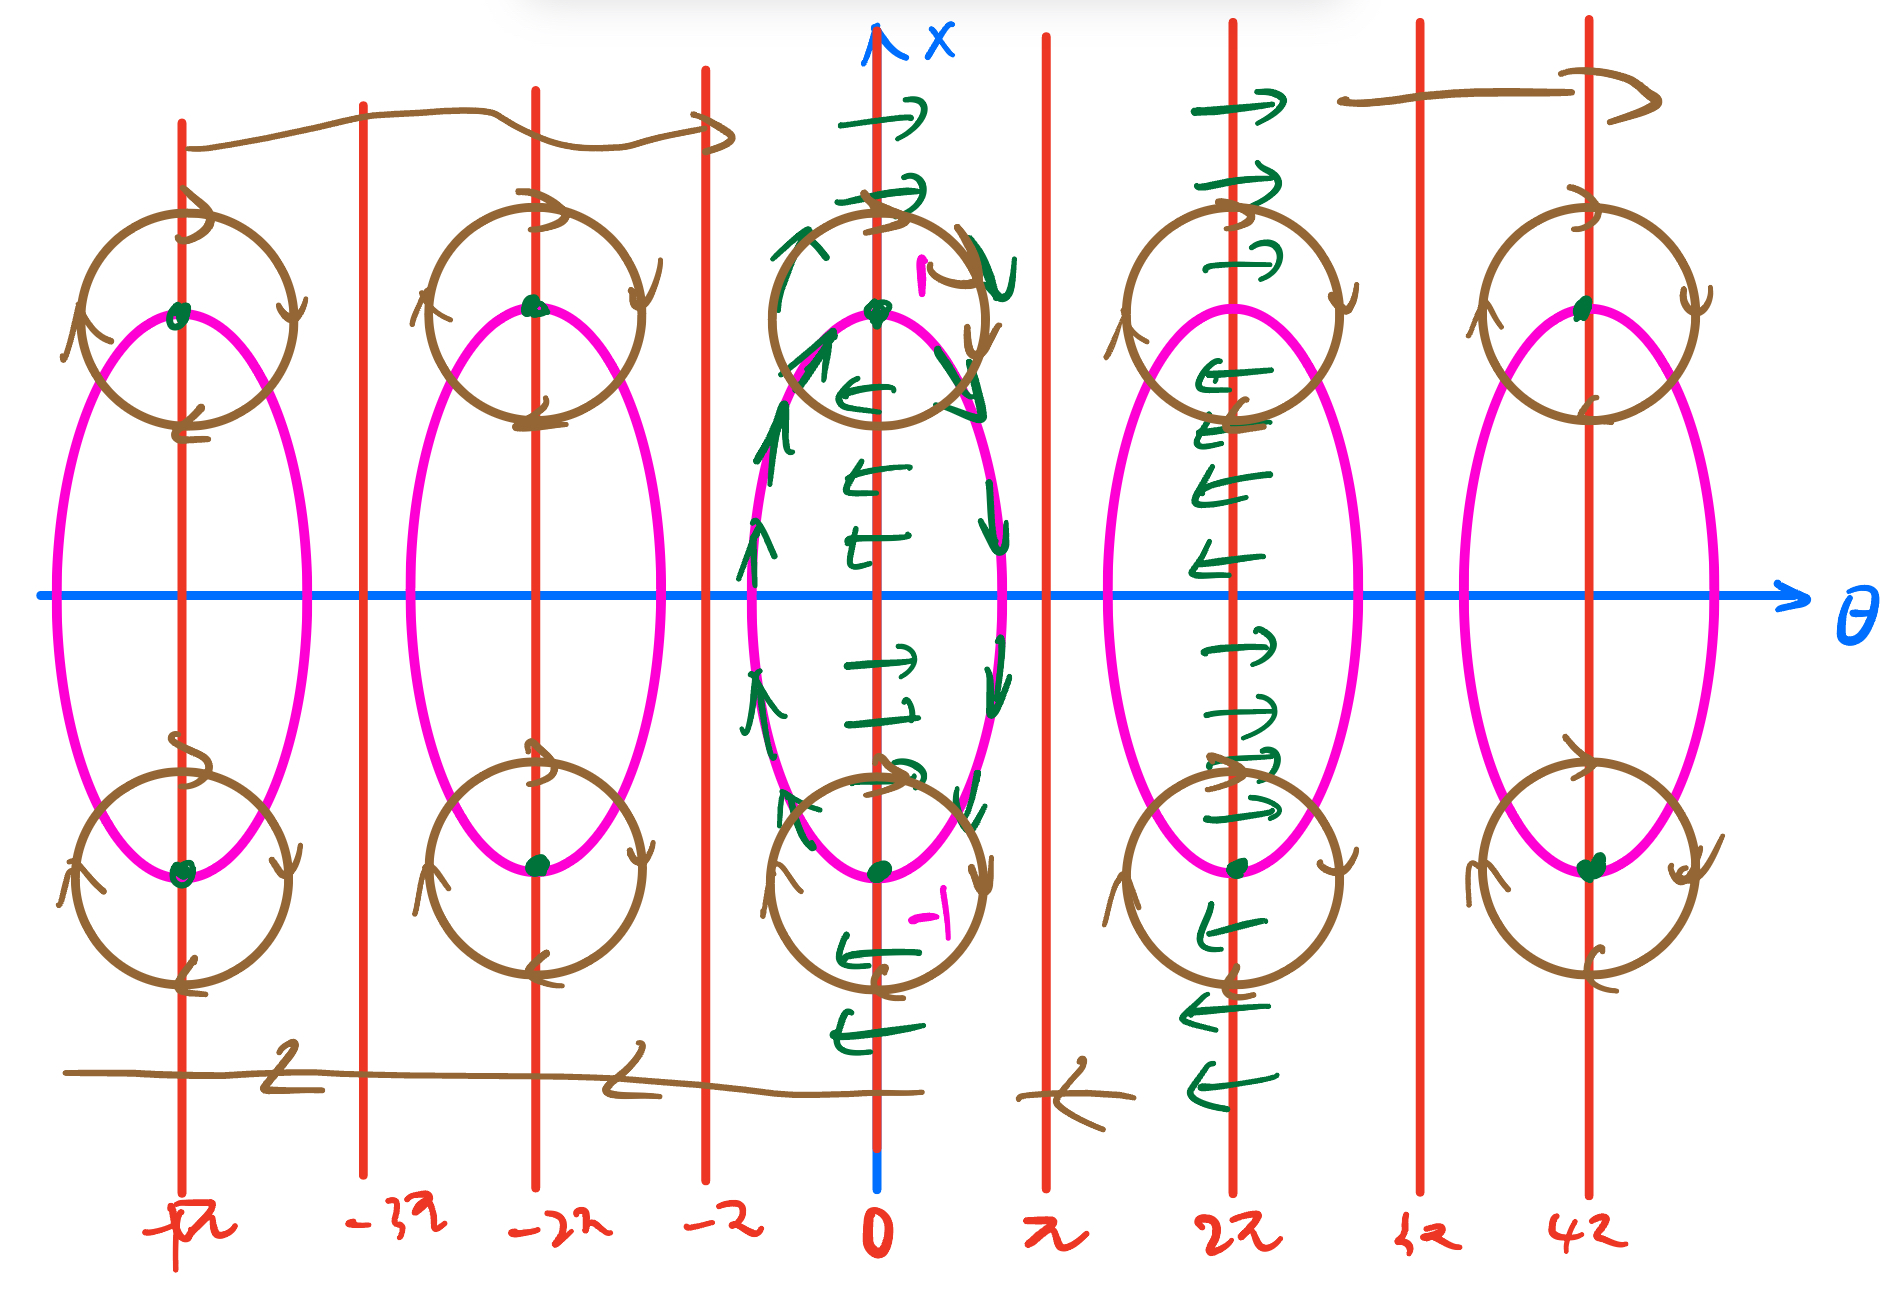
\includegraphics[width=1\linewidth]{1b.jpeg}
				\caption{Phase portrait of the system}
			\end{figure}
		
		\item When $\theta(0) =0, x(0) =1/2$ the glider will fly in a circle with radius $1/2$.\\
			When $\theta(0) =0, x(0) =2$ the glider will fly along around the trajectory $x=2$ and keep flying far away.
	\end{enumerate}




\section*{Problem 2}
For the system
\[ \begin{cases} \dot{x} = \sin y \\ \dot{y} = \sin x \end{cases} \]
\begin{enumerate}[(a)]
	\item Show that the system is invariant under the mappings
	
	\begin{enumerate}[(i)]
		\item  $(t, x, y) \mapsto (-t, x, -y)$. Let $\dot{x} = f(x,y)$ and $\dot{y} = g(x,y)$, then we have 
		\[ \begin{cases} f(x,-y) = \sin -y =- \sin y = -f(x,y) \\ g(x,-y) = \sin x = g(x,y) \end{cases} \]
		Thus, the system is invariant under the mapping $(t, x, y) \mapsto (-t, x, -y)$.
	
		\item $(t, x, y) \mapsto (t, -x, y)$. Let $\dot{x} = f(x,y)$ and $\dot{y} = g(x,y)$, then we have
		\[ \begin{cases} f(-x,y) = \sin y = f(x,y) \\ g(-x,y) = \sin -x = -\sin x = -g(x,y) \end{cases} \]
		Thus, the system is invariant under the mapping $(t, x, y) \mapsto (t, -x, y)$.
	\end{enumerate}

	\item Find all the fixed points of the system.\\
		When $\dot{x} =0$, $\sin y =0$, thus $y = n\pi$, $n\in \mathbb{Z}$. When $\dot{y}=0$, $\sin x =0$, thus $x = n\pi$, $n\in \mathbb{Z}$. Thus, we have fixed points $(x, y) = (n\pi, m\pi)$, $n, m\in \mathbb{Z}$. The Jacobian matrix is
		\[ J = \begin{bmatrix} 0 & \cos y \\ \cos x & 0 \end{bmatrix} \]
		Since this system is time-reversible, we only consider the first quadrant where all the $x,y \geq 0$. When $x=y$, we can get $\tau = 0$, $\Delta = - \cos x^2 <0$ and the fixed point is a saddle. When $(x,y) = (0, n\pi)$, we can get $\tau =0$, $\Delta = (-1)^n <0$ when $n$ is odd and $\Delta = (-1)^n >0$ when $n$ is even. Thus, the fixed point is a saddle when $n$ is odd and a center when $n$ is even. Thus, we have the following phase portrait
		\begin{figure}[H]
			\centering
			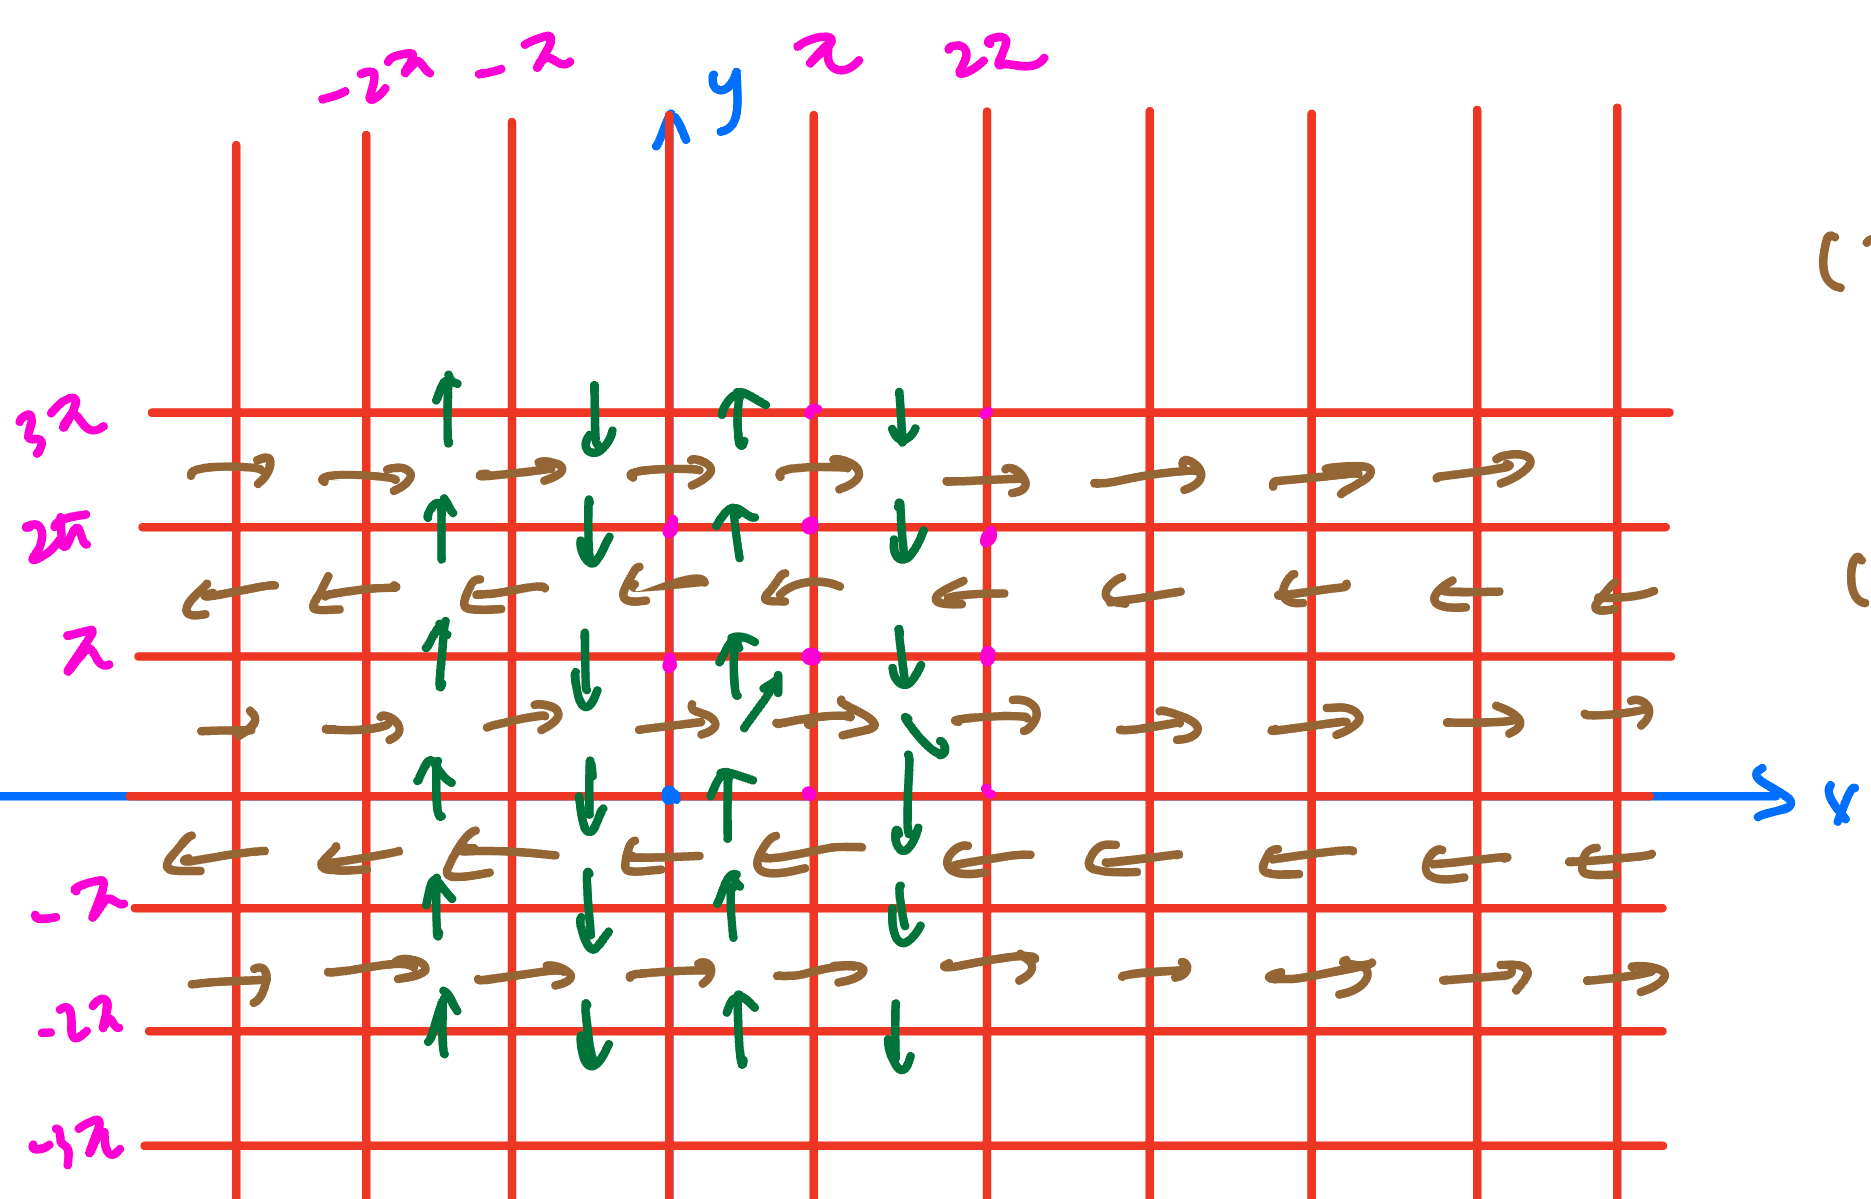
\includegraphics[width=0.7\linewidth]{2b.jpeg}
			\caption{Phase portrait of the system}
		\end{figure}

\end{enumerate}






\section*{Problem 3}
Determine the index of the following fixed points at $(0, 0)$:

\begin{enumerate}[(a)]
	\item $\dot{x} = y-x, \quad \dot{y}=x^2$ \\
		We have
		\[ J = \begin{bmatrix} -1 & 1 \\ 2x & 0 \end{bmatrix} \]
		Thus, we have fixed point $(0, 0)$
		\[ J(0, 0) = \begin{bmatrix} -1 & 1 \\ 0 & 0 \end{bmatrix} \]
		Thus, $\tau = -1$, $\Delta = 0$. The trajectory around $(0, 0)$ cannot be determined by the linearized system. Let's try to use nullcline to plot the phase portrait then choose the unit circle around $(0, 0)$ as closed curve $C$. 
		\begin{figure}[H]
			\centering
			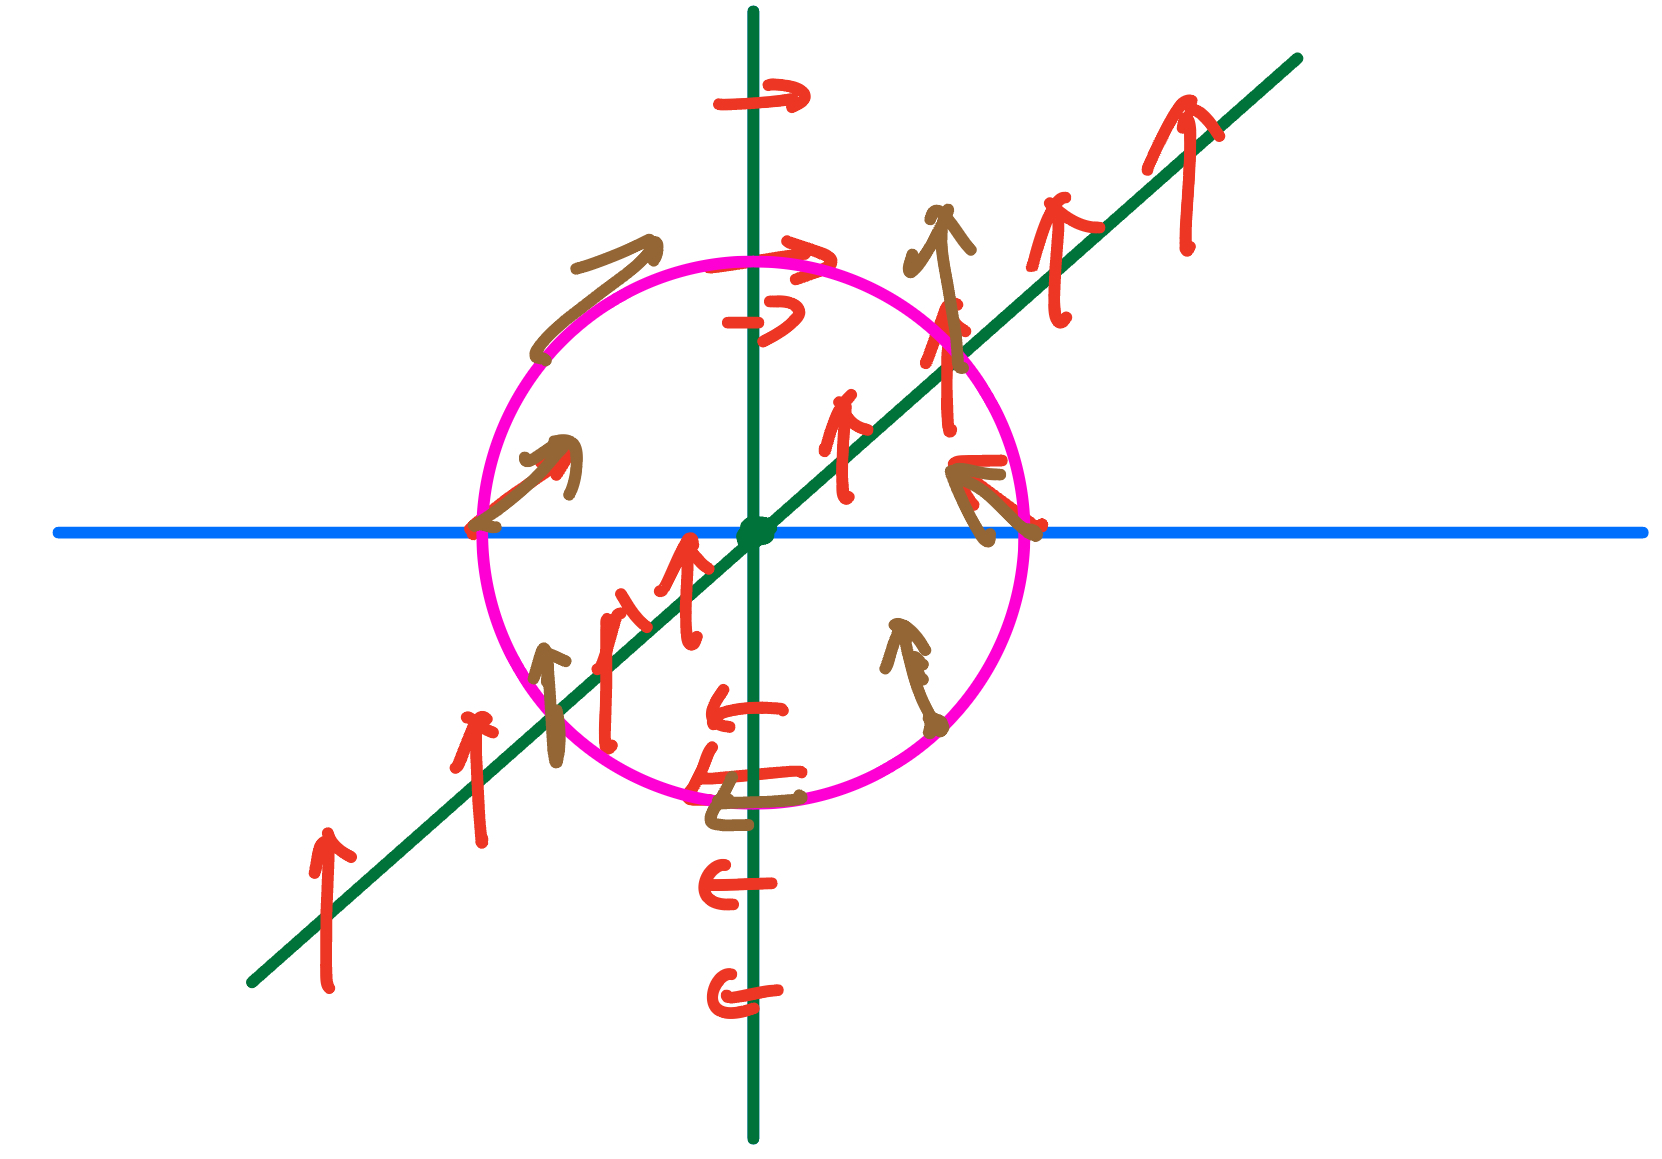
\includegraphics[width=0.7\linewidth]{3a.jpg}
			\caption{Phase portrait of the system}
		\end{figure}
		
		By plot the variation of the vector field of that unit circle, we can see that the index of $(0, 0)$ is $0$.

	\item $\dot{x} = y^3, \quad \dot{y}=x$ \\
		We have
		\[ J = \begin{bmatrix} 0 & 3y^2 \\ 1 & 0 \end{bmatrix} \]
		Thus, we have fixed point $(0, 0)$
		\[ J(0, 0) = \begin{bmatrix} 0 & 0 \\ 1 & 0 \end{bmatrix} \]
		Thus, $\tau = 0$, $\Delta = 0$. The trajectory around $(0, 0)$ cannot be determined by the linearized system. Let's try to use nullcline to plot the phase portrait then choose the unit circle around $(0, 0)$ as closed curve $C$. 
		\begin{figure}[H]
			\centering
			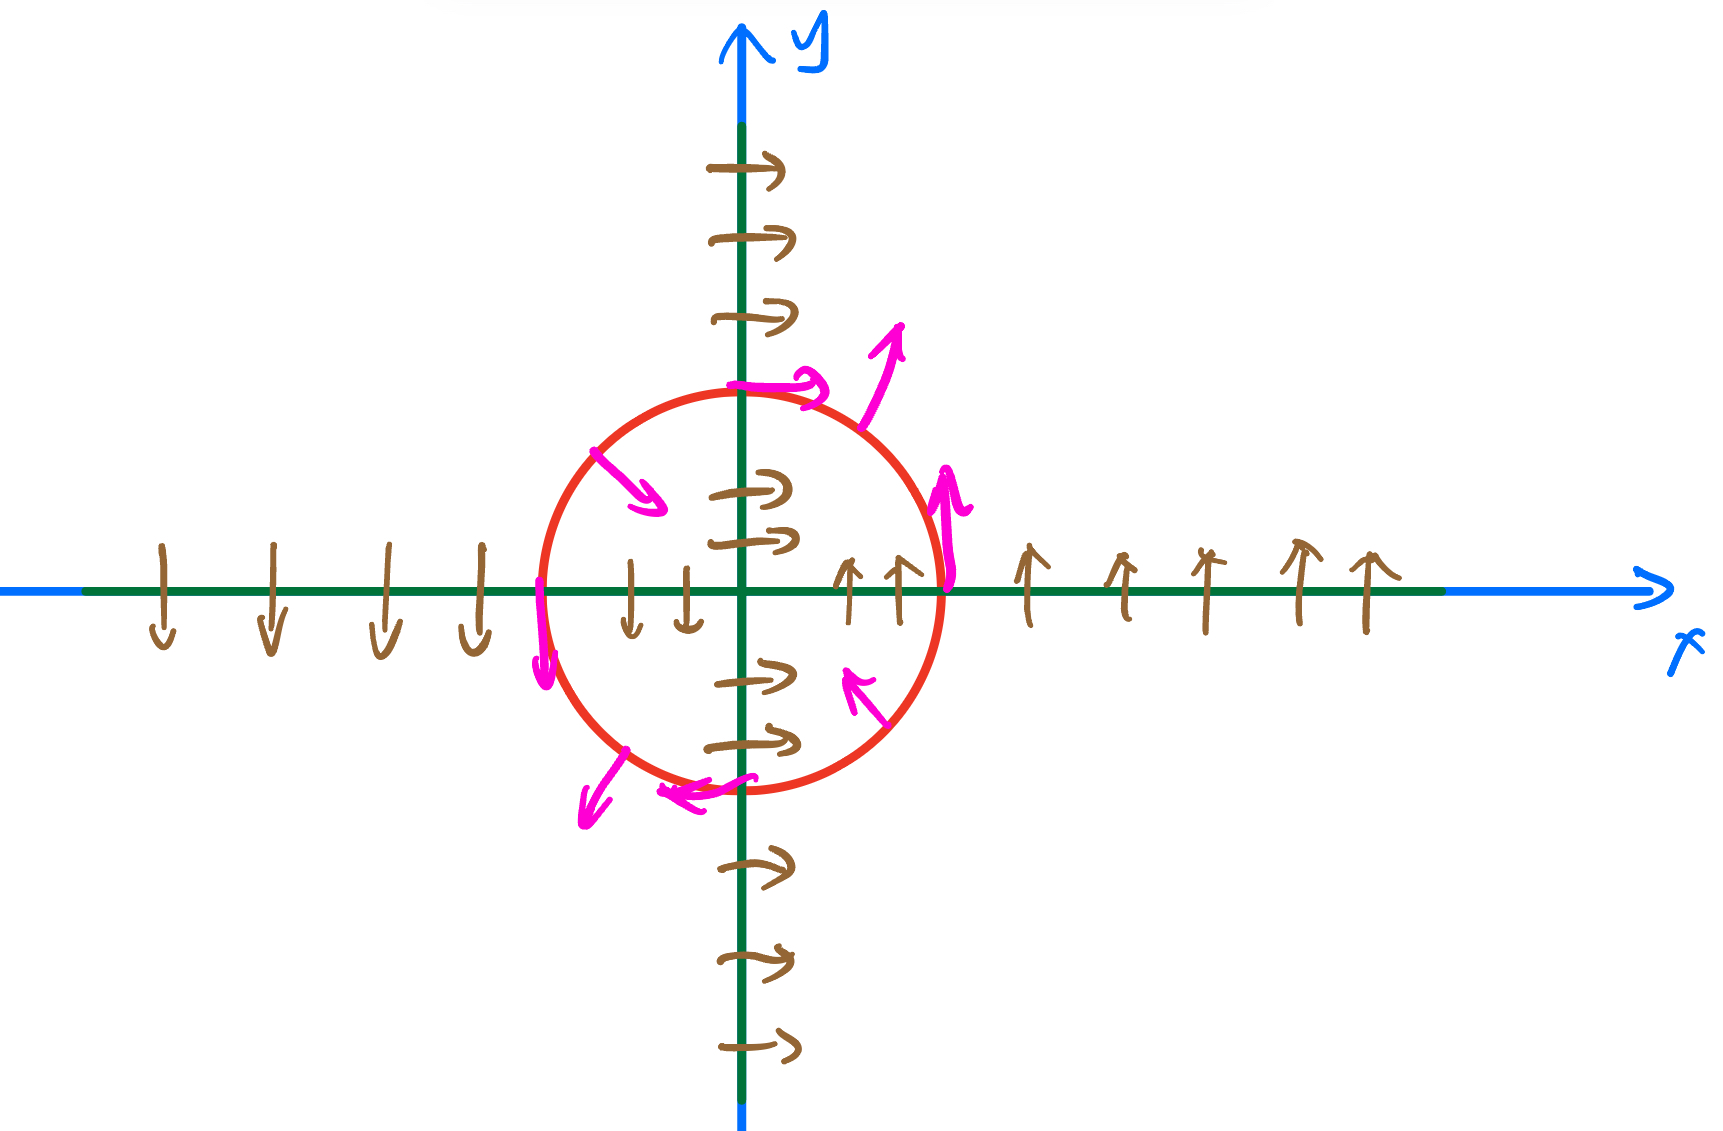
\includegraphics[width=0.7\linewidth]{3b.jpeg}
			\caption{Phase portrait of the system}
		\end{figure}
		By testing the variation of the vector field of that unit circle, we can see that the index of $(0, 0)$ is $-1$.
		

	\item $\dot{x} = xy$, $\dot{y} = x+y$. \\
		We have
		\[ J = \begin{bmatrix} y & x \\ 1 & 1 \end{bmatrix} \]
		Thus, we have fixed point $(0, 0)$
		\[ J(0, 0) = \begin{bmatrix} 0 & 0 \\ 1 & 1 \end{bmatrix} \]
		The two vectors are not linearly independent, thus we cannot determine the index of $(0, 0)$ by using the linearized system. Let's try to use nullcline to plot the phase portrait then choose the unit circle around $(0, 0)$ as closed curve $C$. 
		\begin{figure}[H]
			\centering
			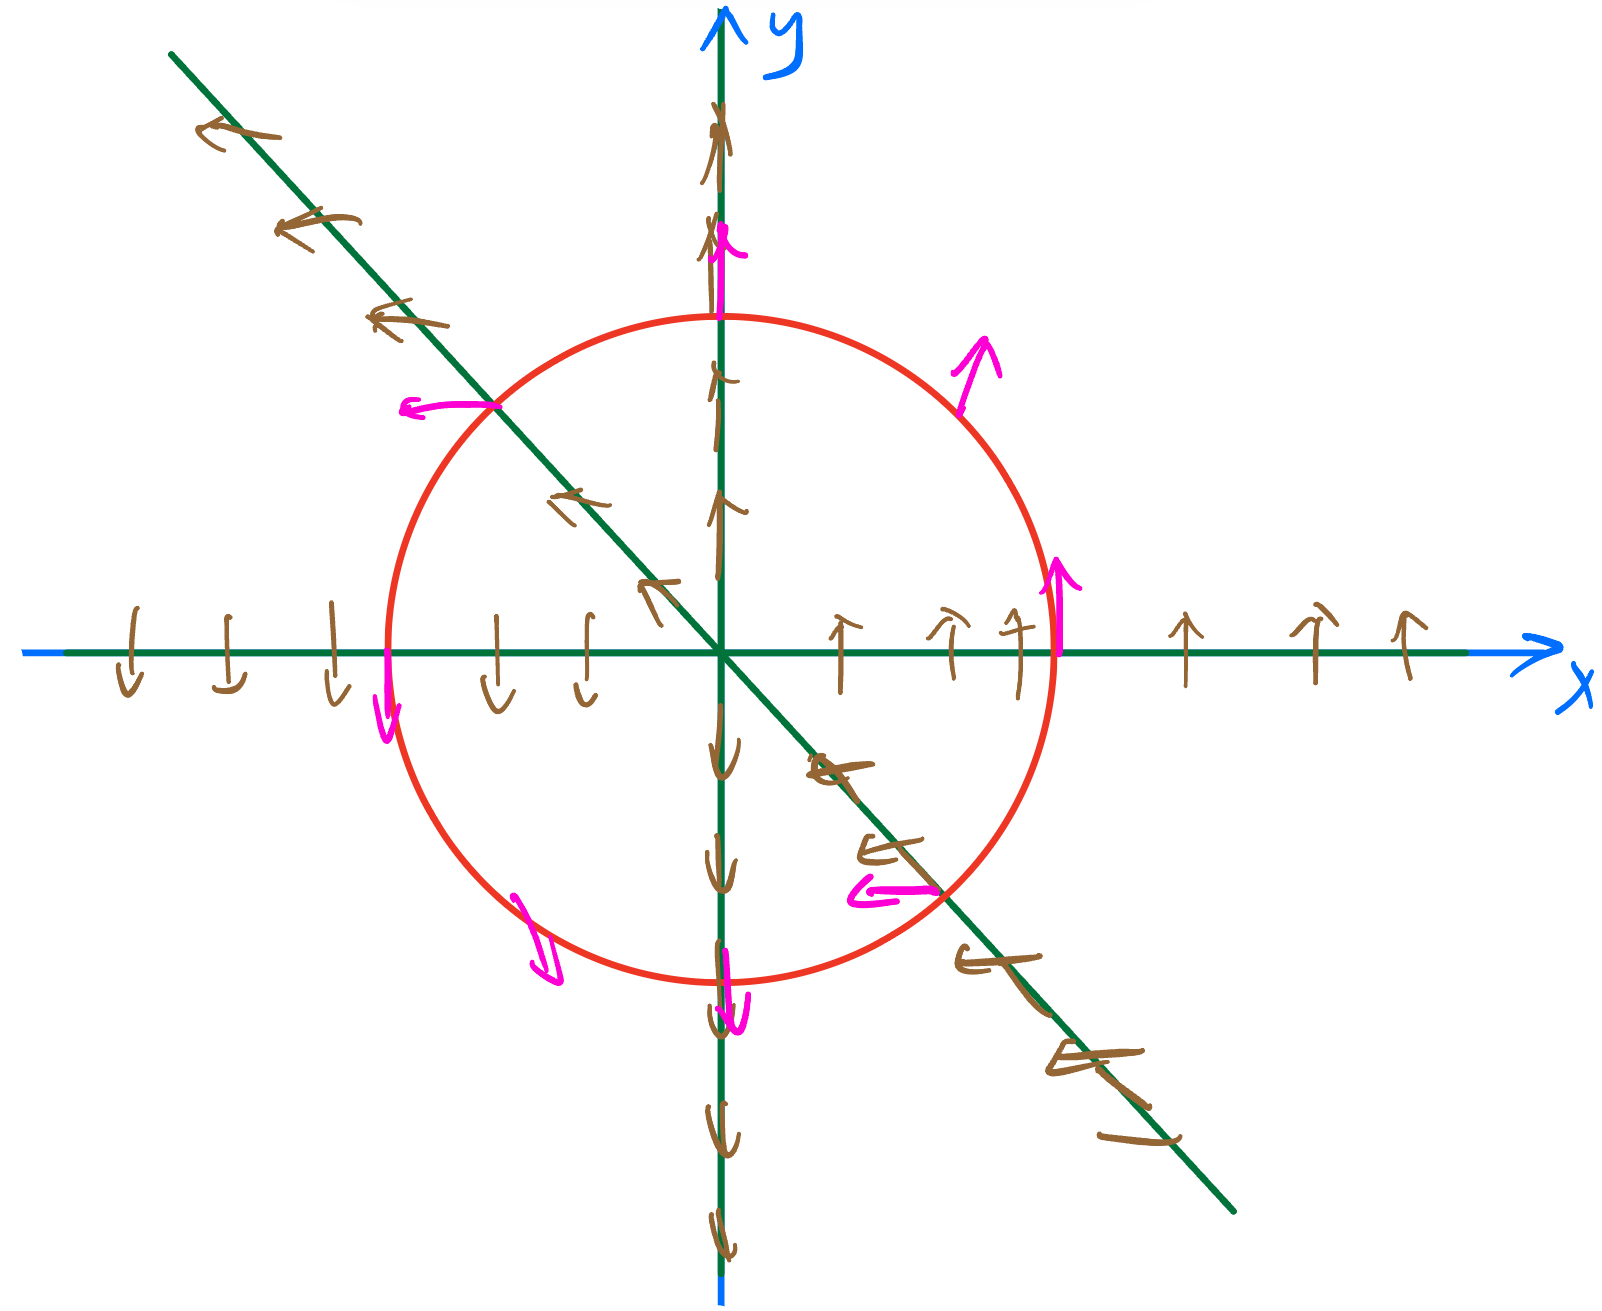
\includegraphics[width=0.7\linewidth]{3c.jpeg}
			\caption{Phase portrait of the system}
		\end{figure}
		By testing the variation of the vector field of that unit circle, we can see that the index of $(0, 0)$ is $0$.
\end{enumerate}

\section*{Problem 4}
\begin{proof}
By theorem 6.8.2 in Strogatz, any closed orbit in the phase plane must enclose fixed points whose indices sum to $+1$. Thus, we have
\[NI_N + FI_F+ CI_C + SI_S = 1\]
Since the The $S$ is saddles the index is $-1$, we have
\[NI_N + FI_F+ CI_C -S = 1\]
Thus, we have
\[N + F + C = 1+ S.\]

\end{proof}










\end{document}

